\documentclass[11pt,a4paper]{article}
\usepackage[margin=16mm]{geometry}
\usepackage[T1]{fontenc}\usepackage{lmodern}\usepackage{microtype}
\usepackage{xcolor,booktabs,tabularx,array,amsmath,enumitem,titlesec,tcolorbox,tikz}
\usetikzlibrary{arrows.meta,decorations.pathmorphing,positioning,calc}
\usepackage[hidelinks]{hyperref}
\setlength{\parindent}{0pt}\setlength{\parskip}{4pt}
\setlist[itemize]{leftmargin=5mm,itemsep=2pt,topsep=2pt}
\setlist[enumerate]{leftmargin=6mm,itemsep=2pt,topsep=2pt}
\titlespacing*{\section}{0pt}{10pt}{4pt}\titlespacing*{\subsection}{0pt}{7pt}{3pt}
\titleformat*{\section}{\large\bfseries}\titleformat*{\subsection}{\normalsize\bfseries}
\definecolor{ink}{HTML}{1D1D1F}\definecolor{muted}{HTML}{6E6E73}\definecolor{blue}{HTML}{0071E3}\definecolor{soft}{HTML}{F5F5F7}\definecolor{line}{HTML}{D2D2D7}\definecolor{warn}{HTML}{FFF3CD}
\color{ink}
\newtcolorbox{keybox}[1]{colback=soft,colframe=line,boxrule=.5pt,arc=2mm,title={#1},fonttitle=\bfseries,coltitle=ink,left=3mm,right=3mm,top=2mm,bottom=2mm}
\newtcolorbox{mistakebox}[1]{colback=warn,colframe=orange!60!black,boxrule=.6pt,arc=2mm,title={#1},fonttitle=\bfseries,coltitle=ink,left=3mm,right=3mm,top=2mm,bottom=2mm}
\newcommand{\unit}[1]{\,\mathrm{#1}}
\begin{document}
\begin{center}
{\LARGE\bfseries GCSE Physics --- Waves, Sound \& Spectrum Review}\par\vspace{2mm}
{\color{muted}Student: Phuc Nguyen \quad Tutor: Alex Kealy \quad Date: 2026-07-19}\par
{\small\color{muted}Source: Loom recording (full video analysis) + transcript}
\end{center}

\begin{keybox}{How to use this lecture-replacement guide}
The lesson began with Alex asking for a \textbf{brain dump}: write everything remembered about waves before opening questions. Use the same method now. On blank paper, write the four quantities $A,\lambda,f,T$, the two equations $v=f\lambda$ and $T=1/f$, the sound and electromagnetic-wave facts, and the EM order. Then compare with the guide. Retrieval before rereading exposes gaps much more reliably than passive highlighting.
\end{keybox}

\section*{1. The big picture: waves transfer energy}
Alex briefly described physics as the scientific study of matter, energy and the relationship between them. Waves fit that picture because a wave transfers energy from place to place without carrying material steadily along with it. The particles of a material may oscillate around equilibrium, but they do not travel with the disturbance over long distances. This distinction becomes crucial in the dust-particle question later: the passing sound wave makes the particle vibrate about its original position; it does not sweep the particle continuously to the right.

The lesson's mind map connected sound, wave properties, equations, reflection, refraction, the Doppler effect, the electromagnetic spectrum and ultrasound. These are not isolated facts. The quantities describe the wave, the equations connect them, and the type of wave tells you how the oscillations are oriented relative to energy transfer.

\section*{2. Describing a wave precisely}
\subsection*{Amplitude, wavelength, frequency and period}
On Phuc's transverse-wave sketch, Alex labelled the four core quantities:
\begin{itemize}
\item \textbf{Amplitude, $A$:} maximum displacement from the equilibrium line. It is measured from equilibrium to a crest or from equilibrium to a trough---not from crest to trough.
\item \textbf{Wavelength, $\lambda$:} distance between consecutive points in the same phase, for example crest to next crest or compression to next compression. Its SI unit is the metre.
\item \textbf{Frequency, $f$:} number of complete cycles passing a point each second. Its unit is hertz, where $1\,\mathrm{Hz}=1$ cycle per second.
\item \textbf{Period, $T$:} time for one complete cycle. Its unit is seconds.
\end{itemize}

\begin{center}
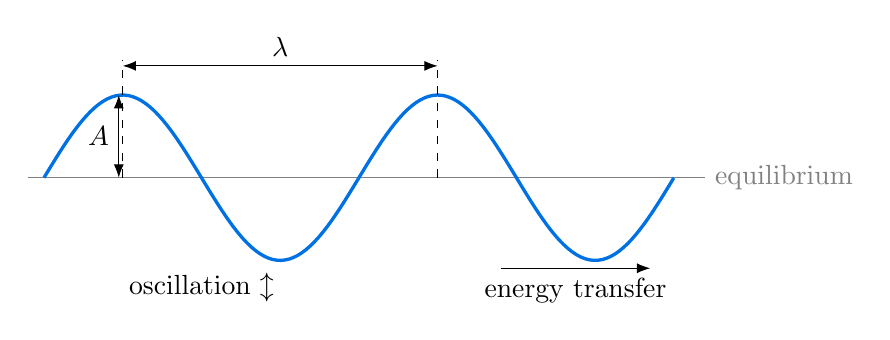
\begin{tikzpicture}[x=1cm,y=1cm,>=Latex]
\draw[gray] (-.2,0)--(8.4,0) node[right]{equilibrium};
\draw[very thick,blue,domain=0:8,samples=150] plot (\x,{1.05*sin(90*\x)});
\draw[<->] (.95,0)--(.95,1.05) node[midway,left]{$A$};
\draw[<->] (1,1.42)--(5,1.42) node[midway,above]{$\lambda$};
\draw[dashed] (1,0)--(1,1.5);\draw[dashed] (5,0)--(5,1.5);
\node[below] at (2,-1.1){oscillation $\updownarrow$};\draw[->] (5.8,-1.15)--(7.7,-1.15) node[midway,below]{energy transfer};
\end{tikzpicture}
\end{center}

Frequency and period are reciprocals:
\[
\boxed{f=\frac{1}{T}}\qquad\boxed{T=\frac{1}{f}}.
\]
Why? If five cycles happen in one second, each cycle occupies one fifth of a second. More cycles per second means less time per cycle.

\subsection*{Measuring frequency in a ripple tank}
The question asked how to measure the frequency of water waves. Phuc's method was correct: choose a fixed point, time a sensible interval such as $10$ seconds, count the number of complete waves passing, and divide the count by the time. In symbols,
\[
f=\frac{\text{number of complete waves}}{\text{time}}.
\]
Using several seconds rather than trying to time one tiny period reduces the percentage effect of reaction-time error. If the motor makes the bar hit the water more times each second, the source oscillates more often, so the produced frequency \textbf{increases}; Phuc selected this correctly.

\subsection*{Worked example: period at 5 Hz}
The paper supplied $f=5\,\mathrm{Hz}$ and the equation period $=1/$frequency. Alex wrote the rearranged relationship explicitly:
\[
T=\frac{1}{f}=\frac{1}{5}=0.2\unit{s}.
\]
The unit must be seconds, not metres or metres per second. A sense check helps: five equally timed waves fit into one second, so each must last less than one second; $0.2\,\mathrm{s}$ is reasonable.

\begin{mistakebox}{Common mistake: confusing amplitude and wavelength}
In the labelled-wave multiple choice, K represented the distance from equilibrium to a crest, so Phuc correctly chose K for amplitude. A crest itself is not an amplitude, and a horizontal crest-to-crest distance is wavelength. If a diagram is unfamiliar, first draw or identify the equilibrium line.
\end{mistakebox}

\section*{3. Wave speed and the equation triangle}
Wave speed, frequency and wavelength are related by
\[
\boxed{v=f\lambda}.
\]
The equation says that each cycle advances the pattern by one wavelength, and $f$ cycles occur every second. Therefore the pattern covers $f\lambda$ metres per second. A useful triangle is:
\begin{center}
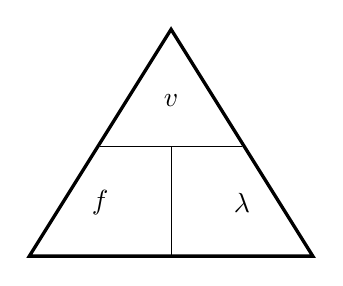
\begin{tikzpicture}[scale=.9]
\draw[very thick] (0,0)--(4,0)--(2,3.2)--cycle;\draw (1,1.55)--(3,1.55);\draw (2,0)--(2,1.55);
\node[font=\bfseries] at (2,2.2){$v$};\node[font=\bfseries] at (1,0.75){$f$};\node[font=\bfseries] at (3,0.75){$\lambda$};
\end{tikzpicture}
\end{center}
Cover the required quantity: $v=f\lambda$, $f=v/\lambda$, or $\lambda=v/f$. The triangle is only a memory aid; always write the equation before substitution and check units.

\subsection*{Worked example: sound wavelength}
For a sound wave with $f=6600\,\mathrm{Hz}$ and $v=330\,\mathrm{m\,s^{-1}}$, Phuc correctly wrote
\[
\lambda=\frac{v}{f}=\frac{330}{6600}=0.050\unit{m}.
\]
The selected unit is metres. The answer is $5.0$ cm, which makes sense because a high-frequency sound has a short wavelength at a fixed speed.

\subsection*{Worked example: the standing-wave trap}
The diagram showed a vibrating string of length $80$ cm, frequency $55$ Hz, and \textbf{two complete wave patterns} across the labelled length. Phuc initially wrote $\lambda=80\,\mathrm{cm}=0.8\,\mathrm{m}$. Alex challenged the interpretation: ``How many wavelengths can you see?'' Phuc answered two. Therefore
\[
2\lambda=80\unit{cm},\qquad \lambda=40\unit{cm}=0.40\unit{m},
\]
then
\[
v=f\lambda=55\times0.40=22\unit{m\,s^{-1}}.
\]

\begin{mistakebox}{Why the first route fails}
The printed length is not automatically one wavelength. Count cycles or use the node/antinode pattern shown. Substituting $0.8$ m would double the wavelength and therefore double the speed to an incorrect $44\,\mathrm{m\,s^{-1}}$. Before using $v=f\lambda$, annotate the diagram with ``number of wavelengths $\times\lambda=$ total length.''
\end{mistakebox}

\section*{4. Transverse and longitudinal waves}
The type of wave is defined by comparing the direction of oscillation with the direction of energy transfer.
\begin{itemize}
\item \textbf{Transverse:} oscillations are perpendicular to energy transfer. Electromagnetic waves are transverse.
\item \textbf{Longitudinal:} oscillations are parallel to energy transfer. Sound in air is longitudinal and contains alternating compressions and rarefactions.
\end{itemize}

\begin{center}
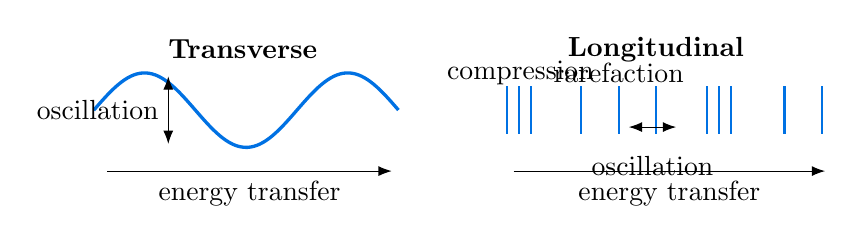
\begin{tikzpicture}[>=Latex,scale=.86]
\node[font=\bfseries] at (2.2,2.9){Transverse};
\draw[very thick,blue,domain=0:4.5,samples=100] plot (\x,{2+0.55*sin(120*\x)});
\draw[->] (0.2,1.1)--(4.4,1.1) node[midway,below]{energy transfer};\draw[<->] (1.1,1.5)--(1.1,2.5) node[midway,left]{oscillation};
\begin{scope}[xshift=6.1cm]
\node[font=\bfseries] at (2.2,2.9){Longitudinal};
\foreach \x in {0,.18,.36,1.1,1.65,2.2,2.95,3.13,3.31,4.1,4.65}{\draw[blue,thick] (\x,1.65)--(\x,2.35);}
\node at (.2,2.55){compression};\node at (1.65,2.55){rarefaction};
\draw[->] (0.1,1.1)--(4.7,1.1) node[midway,below]{energy transfer};\draw[<->] (1.8,1.75)--(2.5,1.75) node[midway,below,yshift=-7pt]{oscillation};
\end{scope}
\end{tikzpicture}
\end{center}

In the dust-particle question, the sound travelled to the right. Phuc first suggested perpendicular motion, mixing up the transverse definition. Alex said ``so close'', and Phuc self-corrected to parallel. The correct option showed the dust vibrating left and right about its original position. It does not move steadily with the wave because the particles pass energy through local oscillations.

\section*{5. Sound needs matter}
Sound is a mechanical wave: it consists of vibrations of material particles. It can travel through gases, liquids and solids, but not through a vacuum because a vacuum contains no particles to pass on the vibration.

The media question listed air, glass, water, mercury and vacuum. Phuc immediately excluded the vacuum and accepted air, but initially doubted glass because he thought fixed atoms could not vibrate. Alex used a concrete analogy: put your ear against a window and tap the glass. The sound reaches your ear through the solid. The particles in a solid are held in fixed average positions, but they can still vibrate around those positions and transfer the disturbance. Alex added that sound travels faster in solids. The lesson's final answer was therefore all listed material media except the vacuum.

\begin{keybox}{Sound and ultrasound facts from the brain dump}
Typical speed of sound in air was recalled as about $330\,\mathrm{m\,s^{-1}}$. Human hearing was used as approximately $20$ Hz to $20{,}000$ Hz. \textbf{Ultrasound} has frequency above $20{,}000$ Hz and can be used for echo-based imaging and industrial applications. The key property is not that ultrasound is a different kind of wave: it is sound above the upper human hearing limit.
\end{keybox}

\section*{6. Echoes and sonar: separate path length from depth}
The boat question gave an ultrasound speed in water of $1500\,\mathrm{m\,s^{-1}}$ and a detected reflection $0.40$ s after emission. Phuc began correctly with
\[
s=vt=1500\times0.40=600\unit{m},
\]
but called $600$ m the seabed depth. This is the total distance travelled by the pulse: down from the boat to the seabed and back to the detector. Alex prompted him to reread the exact question. Once he distinguished the requested one-way depth from the measured round trip, Phuc gave
\[
d=\frac{s}{2}=\frac{600}{2}=300\unit{m}.
\]

\begin{center}
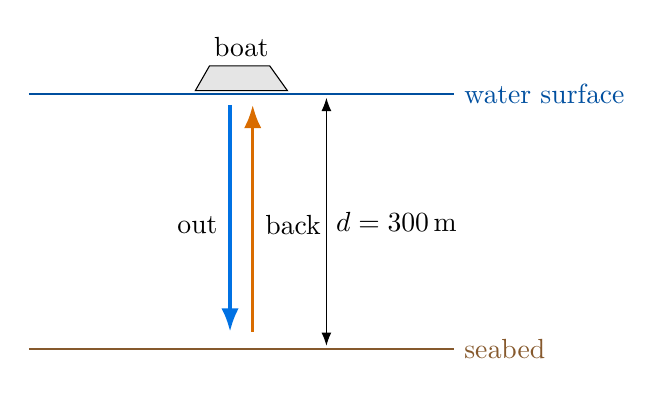
\begin{tikzpicture}[>=Latex,scale=.9]
\draw[blue!70!black,thick] (-3,2)--(3,2) node[right]{water surface};\draw[brown!70!black,thick] (-3,-1.6)--(3,-1.6) node[right]{seabed};
\draw[fill=gray!20] (-.65,2.05)--(.65,2.05)--(.4,2.4)--(-.45,2.4)--cycle;\node[above] at (0,2.4){boat};
\draw[very thick,blue,-Latex] (-.16,1.85)--(-.16,-1.35);\draw[very thick,orange!85!black,-Latex] (.16,-1.35)--(.16,1.85);
\draw[<->] (1.2,1.95)--(1.2,-1.55) node[midway,right]{$d=300\,\mathrm{m}$};
\node[left] at (-.2,.15){out};\node[right] at (.2,.15){back};
\end{tikzpicture}
\end{center}

\begin{mistakebox}{Alex's exam-reading rule}
Look for whether the question asks for ``there and back'' or ``just that distance''. A reflection time usually covers the complete echo path. Either halve the total distance after $s=vt$, or halve the time first and calculate $d=v(t/2)$. Never halve both.
\end{mistakebox}

\section*{7. Hearing-range table: test every condition}
The lesson table gave:
\begin{center}
\begin{tabular}{lc}\toprule Animal & Hearing range / Hz\\\midrule dog & $70$--$45{,}000$\\ bat & $2000$--$110{,}000$\\ elephant & $10$--$12{,}000$\\\bottomrule\end{tabular}
\end{center}
Human hearing was taken as $20$--$20{,}000$ Hz. Four statements were tested.
\begin{enumerate}
\item The highest human pitch ($20{,}000$ Hz) \emph{can} be heard by a dog because it lies between $70$ and $45{,}000$ Hz, so the statement saying it cannot is false.
\item The lowest elephant pitch is $10$ Hz, below the human minimum of $20$ Hz, so it cannot also be heard by a human. False.
\item Phuc initially marked $500$ Hz as audible to all four groups. Alex and the revealed solution caught the missed constraint: $500$ Hz is below the bat minimum of $2000$ Hz. False.
\item At a common wave speed, $\lambda=v/f$, so shortest wavelength corresponds to highest frequency. Bats, not elephants, have the highest upper frequency in the table. False.
\end{enumerate}
Therefore \textbf{none of the statements is correct}. The reusable strategy is to write each required range beside the proposed frequency and test every named animal. A statement with ``all'' fails if even one range fails.

\section*{8. Electromagnetic spectrum and linked ideas}
Phuc recalled the sequence
\[
\boxed{\text{Radio, Microwave, Infrared, Visible, Ultraviolet, X-ray, Gamma}}.
\]
All electromagnetic waves are transverse, travel at $3\times10^8\,\mathrm{m\,s^{-1}}$ in a vacuum, and can propagate through a vacuum. Along the order from radio to gamma, frequency increases and wavelength decreases. Alex also sang a mnemonic song in the review; the key exam requirement is still the full, correctly ordered seven-band sequence.

The brain dump also captured:
\begin{itemize}
\item \textbf{Reflection:} draw a normal perpendicular to the surface and measure both angles from it; angle of incidence equals angle of reflection, $i=r$.
\item \textbf{Refraction:} a ray changes direction at a boundary when wave speed changes; Phuc's sketch showed a ray entering the second medium and bending toward the normal.
\item \textbf{Doppler effect:} change in observed frequency due to relative motion between source and observer. In Phuc's car sketch, wavefronts were compressed in front of the moving car and spread behind it, corresponding to higher frequency ahead and lower frequency behind.
\end{itemize}

\begin{keybox}{Scope boundary from Alex}
Alex briefly said electromagnetic waves are produced by oscillating electric and magnetic fields, but deferred the detailed field explanation to a later topic. For this GCSE review, retain the tested properties above; do not replace them with an invented A-level field treatment.
\end{keybox}

\section*{9. Reconstructing the opening brain dump}
The first useful product of the lesson was not a polished set of notes but a map of what Phuc could retrieve unaided. Reconstructing that map is a powerful revision task because each branch asks a different kind of question.

\begin{tabularx}{\linewidth}{>{\bfseries}p{.20\linewidth}X}
\toprule Branch & What Phuc and Alex put on the board\\\midrule
Sound & Longitudinal; needs a medium; speed about $330\,\mathrm{m\,s^{-1}}$ in air; Alex added compressions and rarefactions.\\
Properties & A transverse sketch labelled amplitude $A$, wavelength $\lambda$, frequency $f$ and period $T$; Phuc supplied $f=1/T$.\\
Doppler effect & A moving car with crowded wavefronts in front and spread-out wavefronts behind; change in observed frequency caused by relative source--observer motion.\\
Reflection & Incident ray, reflected ray, dashed normal, angles $i$ and $r$, and the law $i=r$.\\
Refraction & A ray crossing from medium $n_1$ into $n_2$ and bending toward the normal in the drawn case.\\
EM spectrum & R, M, I, V, U, X, G; transverse; $3\times10^8\,\mathrm{m\,s^{-1}}$; can cross a vacuum.\\
Ultrasound & $f>20{,}000$ Hz; echo/imaging; medical and industrial uses.\\\bottomrule
\end{tabularx}

The value of this map is the network of contrasts. Sound and EM waves are both waves, yet sound needs matter while EM waves cross a vacuum. Sound is longitudinal while EM waves are transverse. Reflection keeps the ray in the original medium while refraction concerns crossing a boundary. Frequency and period describe timing; wavelength describes spatial repetition; speed connects the temporal and spatial descriptions.

\subsection*{A disciplined second brain dump}
Try the method in three passes. First, write only branch names from memory. Second, add definitions, units and equations. Third, draw one diagram per branch and annotate it. Use a different colour to correct omissions from this guide. The colour difference is evidence about what must be retrieved again tomorrow; it is not a mark of failure. Alex's opening method worked because it revealed the student's current model before the questions tested individual details.

\section*{10. Why the equations fit together}
It is easy to memorise $T=1/f$, $v=f\lambda$ and $s=vt$ as three unrelated formulas. They are better understood as three views of repeated motion. Frequency tells us how many repeats happen each second. Period tells us how many seconds each repeat takes. Wavelength tells us how far apart repeats are in space. Multiplying repeats per second by metres per repeat gives metres per second:
\[
\frac{\text{cycles}}{\mathrm{s}}\times\frac{\mathrm{m}}{\text{cycle}}=\frac{\mathrm{m}}{\mathrm{s}}.
\]
This unit cancellation is also a diagnostic. If a purported wavelength calculation leaves units of hertz or seconds, the rearrangement is wrong. For $\lambda=v/f$, the units are
\[
\frac{\mathrm{m\,s^{-1}}}{\mathrm{s^{-1}}}=\mathrm{m}.
\]

The equation $s=vt$ is more general: distance is speed multiplied by elapsed time. In the sonar problem the arithmetic was never the difficult physics. The difficult physics was deciding what physical path the elapsed time described. A labelled sketch makes that decision visible. The same habit helps with any echo, radar or reflected-pulse question: draw the outbound and return legs before inserting numbers.

\begin{mistakebox}{A four-line calculation protocol}
\textbf{1. Identify} the required quantity and the path or cycle it represents. \textbf{2. Write} the equation in symbols. \textbf{3. Convert} units before substitution. \textbf{4. Check} magnitude, unit and whether the diagram contains multiple wavelengths or multiple journey legs. The standing-string and sonar corrections both reduce to Step 1.
\end{mistakebox}

\section*{11. Practical thinking from the ripple-tank discussion}
A frequency measurement is an experiment, not just a sentence. A complete method needs an observable event, a reference point, a measured time and a calculation. ``Count waves'' is incomplete unless the counting location and time interval are specified. Choose a fixed point in the tank; count crests crossing that point for ten seconds; calculate frequency by count divided by ten. Repeating the measurement and averaging would make the estimate more reliable, although the lesson's required method centred on timing and counting.

Alex noted later that practical-method questions are hard when the practical has not been physically performed. The appropriate response is not to invent equipment or observations. Translate the definition into measurable quantities. Frequency is cycles per second, so measure cycles and seconds. Period is seconds per cycle, so either time one cycle carefully or measure several and divide. This definition-to-method route works even when the apparatus is unfamiliar.

When the motor bar strikes more often each second, frequency rises because the driving source sets the repetition rate. At a fixed wave speed, $v=f\lambda$ then implies that a higher frequency corresponds to a shorter wavelength. The lesson question only asked for frequency, so do not add an unsupported claim that speed must also increase. Answer the command given, then use equations only if another quantity is requested.

\section*{12. Worked-example audit: what each question was really testing}
\begin{tabularx}{\linewidth}{>{\bfseries}p{.22\linewidth}X X}
\toprule Question & Surface task & Deeper test\\\midrule
Ripple motor & Select increased/decreased/unchanged & Link source oscillations per second to frequency.\\
Measure frequency & Describe a method & Turn the definition ``cycles per second'' into measurements.\\
Period at $5$ Hz & Substitute into $T=1/f$ & Use reciprocal quantities and choose seconds.\\
Amplitude letter & Read a diagram & Measure maximum displacement from equilibrium.\\
Sound wavelength & Use $\lambda=v/f$ & Rearrange, substitute and select metres.\\
Sonar depth & Use $s=vt$ & Distinguish total echo path from one-way depth.\\
Standing string & Use $v=f\lambda$ & Count wavelengths inside the labelled length.\\
Animal hearing & Test statements & Check every range, especially universal claims.\\
Dust particle & Select motion & Separate longitudinal particle oscillation from wave travel.\\
Sound media & Select materials & Understand that solid particles vibrate; vacuum has none.\\\bottomrule
\end{tabularx}

This audit shows why merely memorising final numbers is weak revision. The answers $0.2$ s, $0.050$ m, $300$ m and $22\,\mathrm{m\,s^{-1}}$ matter, but the transferable decisions are reciprocal, rearrangement, round trip and cycle counting. Those decisions are what a differently worded exam question will test.

\section*{13. Formula and decision table}
\begin{tabularx}{\linewidth}{>{\bfseries}p{.25\linewidth}p{.23\linewidth}X}
\toprule Situation & Formula / fact & Decision check\\\midrule
Period from frequency & $T=1/f$ & Hz goes in; seconds comes out.\\
Frequency from period & $f=1/T$ & Count complete cycles per second.\\
Wave calculation & $v=f\lambda$ & Convert cm to m before substitution.\\
Motion / echo & $s=vt$ & Decide whether $s$ is one-way or round-trip.\\
Transverse & oscillation $\perp$ transfer & EM waves.\\
Longitudinal & oscillation $\parallel$ transfer & Sound; compressions and rarefactions.\\
Reflection & $i=r$ & Measure angles from the normal.\\
EM order & R M IR V UV X $\gamma$ & Frequency rises; wavelength falls.\\\bottomrule
\end{tabularx}

\section*{14. Quick-recall summary}
Without looking back, answer these aloud:
\begin{enumerate}
\item Define amplitude and wavelength, and state the unit of each.
\item Explain why $f$ and $T$ are reciprocals.
\item A source oscillates more times per second. What changes?
\item A $6600$ Hz sound travels at $330\,\mathrm{m\,s^{-1}}$. Find $\lambda$.
\item Two wavelengths occupy $80$ cm at $55$ Hz. Find the speed.
\item Describe the particle motion when sound travels right.
\item Why can sound travel through glass but not a vacuum?
\item Why must a $600$ m sonar path produce a $300$ m depth in the lesson example?
\item Why was the claim that $500$ Hz is heard by bats wrong?
\item Recite the EM spectrum and state the direction of frequency and wavelength.
\end{enumerate}

\begin{keybox}{Final exam checklist}
Write the formula before numbers; convert units; identify what the diagram's length really represents; keep particle oscillation separate from wave travel; test every row of a range table; and reread echo questions for one-way versus round-trip distance. These checks target the exact places where the lesson exposed or corrected errors.
\end{keybox}
\end{document}
